\section{Data Preparation · Del euro al coeficiente}

\begin{takeaway}
Tres transformaciones convierten el gasto bruto en una señal que el modelo puede aprender: \textbf{(1)} agrupación de los 8 canales en \textbf{4 grupos} según su mecánica de respuesta, \textbf{(2)} \textit{adstock} con $\alpha$ diferenciado por grupo, y \textbf{(3)} saturación logarítmica (retornos decrecientes). El resto del pipeline se apoya íntegramente en este bloque.
\end{takeaway}

\subsection{De 8 canales a 4 grupos}

La fase exploratoria ya avisó: los ocho canales de inversión están correlacionados entre sí con $\rho$ de Spearman entre 0.83 y 0.96. Traducido: cuando invertimos en uno, solemos invertir en varios a la vez. Para una regresión con restricción \texttt{positive=True} esto es letal — los canales se ``canibalizan'' y el modelo termina anulando varios de ellos arbitrariamente.

\begin{decisionbox}
\textbf{Solución:} agrupar los ocho canales en cuatro grupos con mecánica de respuesta distinta. Cada grupo suma dos canales:

\begin{center}
\begin{tabular}{@{}p{3.3cm} p{6.2cm} p{1.4cm} p{1.4cm}@{}}
\toprule
\textbf{Grupo} & \textbf{Canales que lo forman} & $\boldsymbol{\alpha}$ & \textbf{Lag} \\
\midrule
\textcolor{kmgolddark}{Performance}           & \texttt{paid\_search} + \texttt{social\_paid}  & 0.20 & 0 \\
\textcolor{kmgolddark}{Branding Digital}      & \texttt{display} + \texttt{video\_online}     & 0.50 & 1 \\
\textcolor{kmgolddark}{Offline Medios}        & \texttt{radio\_local} + \texttt{prensa}       & 0.60 & 1 \\
\textcolor{kmgolddark}{Propios y Exterior}    & \texttt{email\_crm} + \texttt{exterior}       & 0.70 & 0 \\
\bottomrule
\end{tabular}
\end{center}

Cuatro grupos con $\alpha$ crecientes (memoria desde 1 semana hasta varios meses) $\rightarrow$ coeficientes estables, intervalos de confianza manejables, y la granularidad que necesita el directivo para tomar decisiones.
\end{decisionbox}

\subsection{Adstock · La memoria publicitaria}

Un anuncio no deja de surtir efecto al día siguiente. El consumidor lo recuerda durante semanas. Se modela así:

\[
A_t = x_{t-\text{lag}} + \alpha \cdot A_{t-1}
\]

donde $x_t$ es la inversión en la semana $t$, $\alpha$ el \textit{decaimiento} semanal, $\text{lag}$ el retardo hasta que empieza el efecto, y $A_t$ el ``stock'' publicitario acumulado.

\begin{itemize}[leftmargin=*, itemsep=1pt]
    \item \textbf{Performance} ($\alpha=0.20$): respuesta casi inmediata, memoria corta (paid search y social responden el mismo día).
    \item \textbf{Branding Digital} ($\alpha=0.50$, lag 1): efecto retardado de una semana y memoria media.
    \item \textbf{Offline Medios} ($\alpha=0.60$, lag 1): radio y prensa penetran con retardo y dejan recuerdo más largo.
    \item \textbf{Propios y Exterior} ($\alpha=0.70$): email CRM e imagen exterior construyen memoria a largo plazo ($\sim$2 meses de vida media).
\end{itemize}

\begin{decisionbox}
\textbf{Los $\alpha$ por grupo se fijan con priors de literatura, no se calibran.} Razón: con correlaciones tan altas entre grupos, la calibración automática converge siempre a la esquina del grid ($\alpha \approx 0.90$, lag $=4$) — una solución matemáticamente óptima pero sin sentido de negocio. Usar priors de literatura mantiene el modelo interpretable.
\end{decisionbox}

\subsection{Saturación · Retornos decrecientes}

Invertir el doble no vende el doble. A partir de cierto punto, cada euro adicional rinde menos. Se modela con un logaritmo:

\[
\mathrm{logadstock}_t = \log\left(1 + \frac{A_t}{k}\right)
\]

donde $k$ es la escala característica de cada grupo (percentil 60 de sus valores positivos). En nuestro caso $k \in [112\text{k}€, 139\text{k}€]$ según el grupo. Esta transformación:

\begin{itemize}[leftmargin=*, itemsep=1pt]
    \item \textbf{suaviza los picos} de inversión (un mes de TV/exterior brutal no tiene un efecto 10$\times$),
    \item \textbf{estandariza las escalas} entre grupos que operan en órdenes de magnitud similares pero no idénticos,
    \item \textbf{introduce la saturación} que más tarde se explotará en el simulador del dashboard.
\end{itemize}

\subsection{Visualización de la transformación}

\begin{figure}[htbp]
\centering
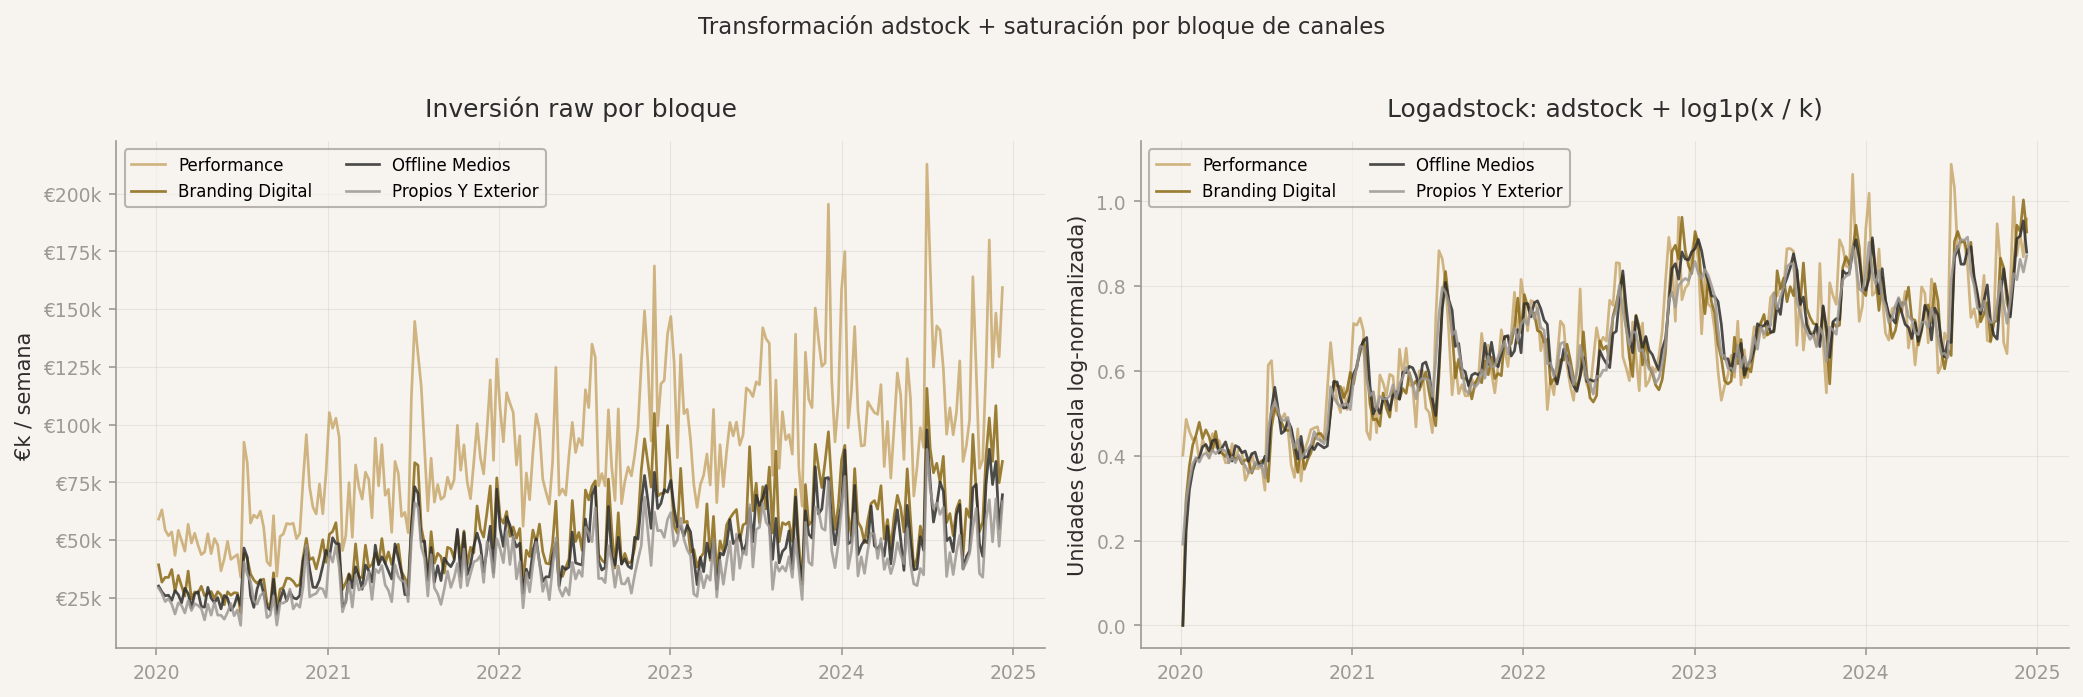
\includegraphics[width=\textwidth]{figures/dp_g1_raw_vs_logadstock.png}
\caption{\textbf{Inversión bruta vs. logadstock por grupo.} Arriba, la inversión semanal bruta de cada grupo: picos puntuales y ceros. Abajo, tras aplicar \textit{adstock} + saturación: señales suaves, persistentes en el tiempo, que reflejan la memoria acumulada de la marca. Estas son las cuatro variables de marketing que verá el modelo.}
\label{fig:dp_raw_vs_log}
\end{figure}

\begin{figure}[htbp]
\centering
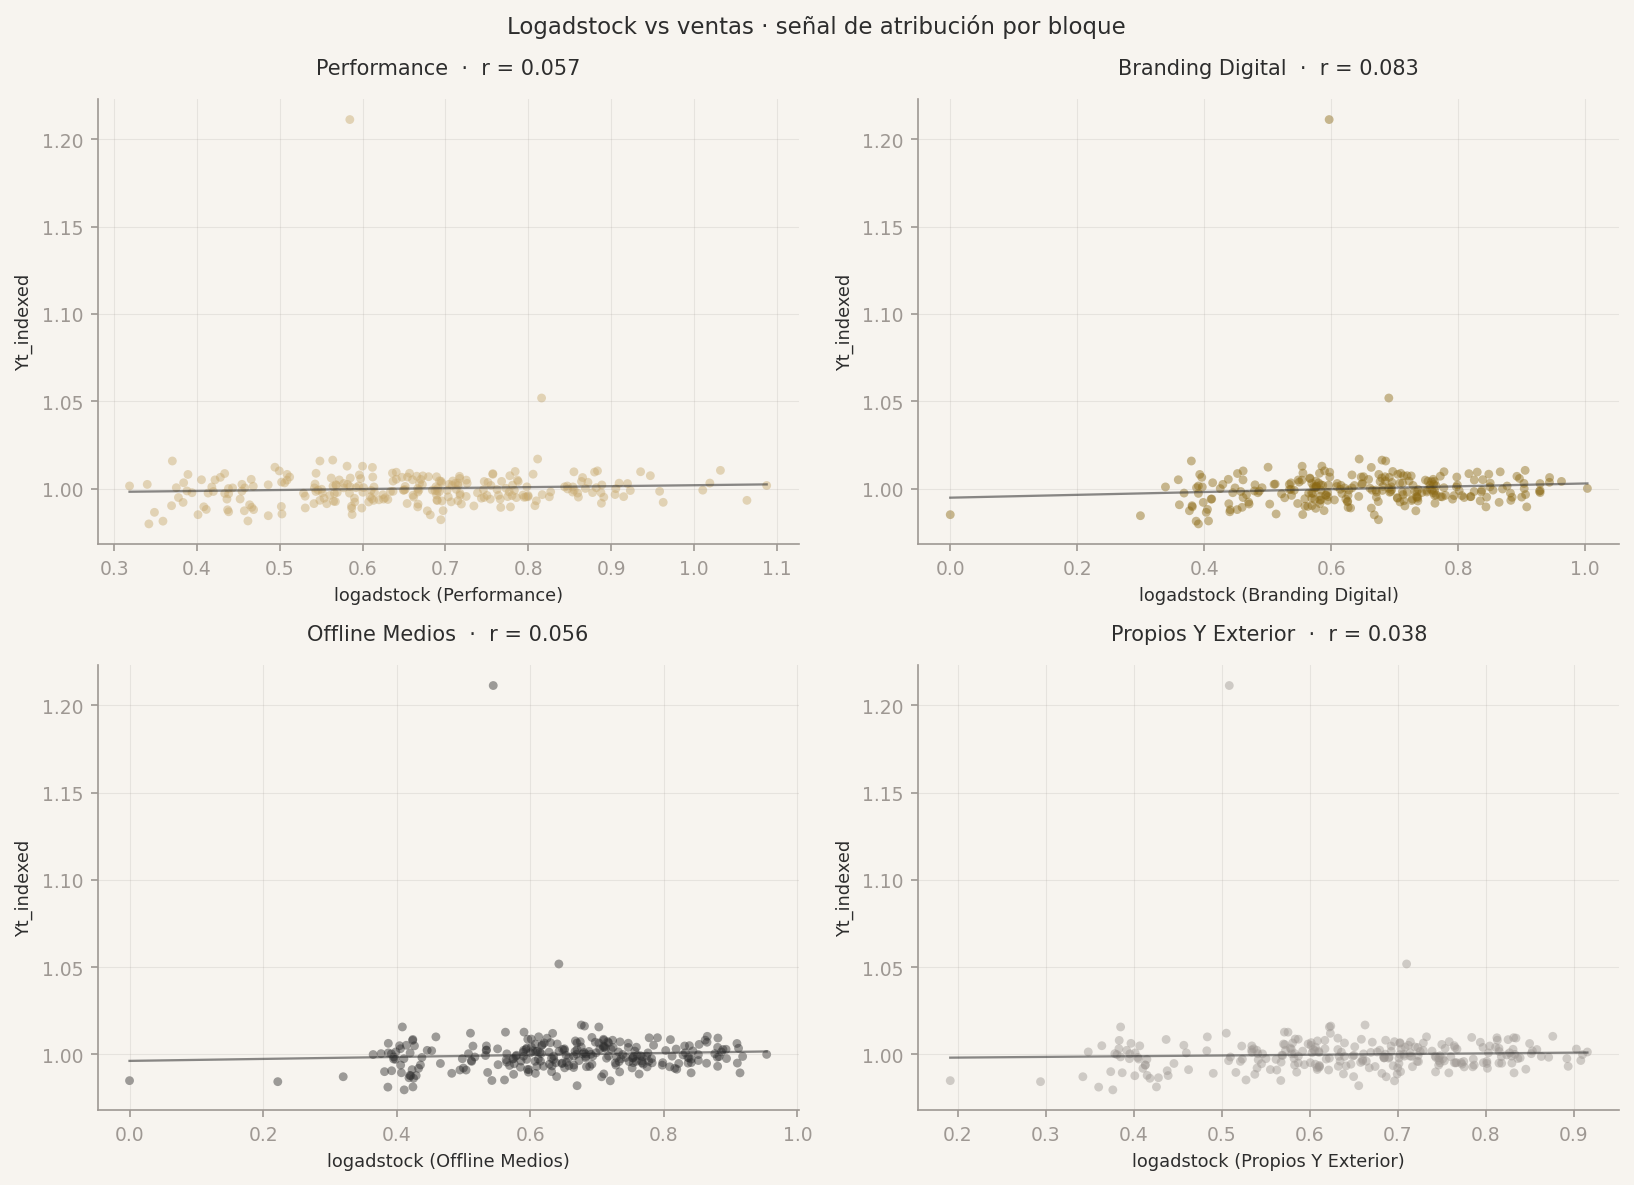
\includegraphics[width=0.95\textwidth]{figures/dp_g2_scatter_senal.png}
\caption{\textbf{Señal logadstock vs. ventas.} Una correlación positiva tras la transformación confirma que la señal de cada grupo co-varía con las ventas en la dirección esperada. Requisito mínimo antes de pasar al modelo: sin esto, no hay nada que aprender.}
\label{fig:dp_scatter}
\end{figure}

\begin{figure}[htbp]
\centering
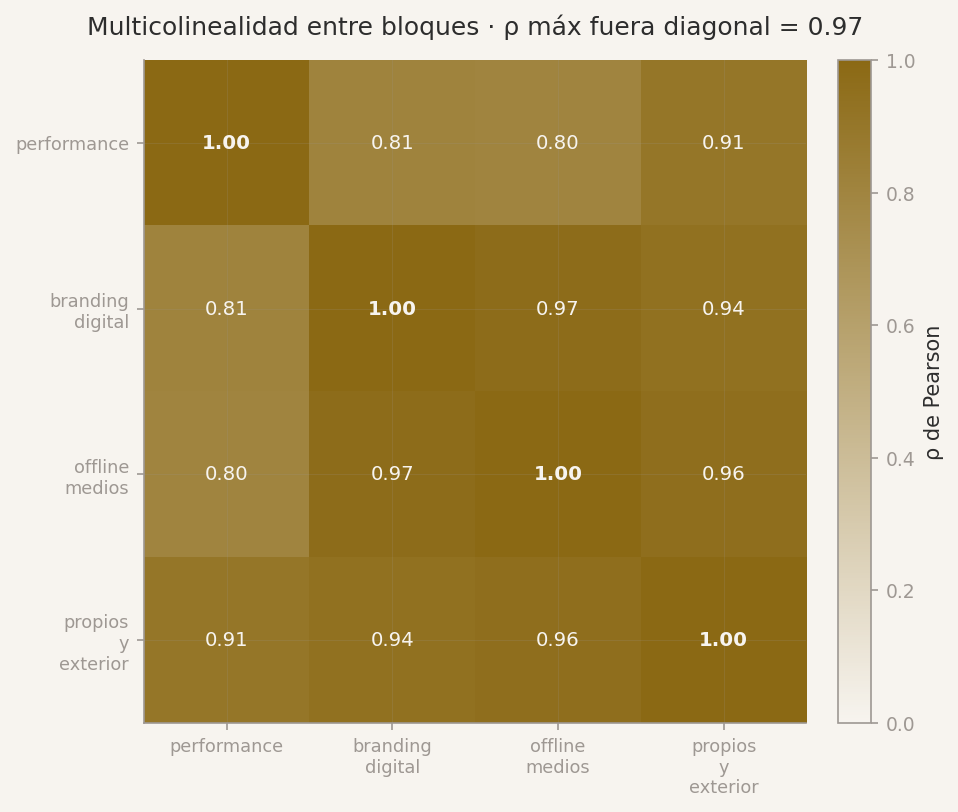
\includegraphics[width=0.8\textwidth]{figures/dp_g3_multicolinealidad.png}
\caption{\textbf{Multicolinealidad entre los 4 grupos transformados.} Tras la agrupación y el adstock con $\alpha$ diferenciado, los cuatro grupos quedan en correlación \textit{manejable}, que es lo que permite a ElasticNet separar la contribución de cada uno.}
\label{fig:dp_multico}
\end{figure}

\subsection{Feature set final}

Tras la preparación, el modelo recibe \textbf{19 variables}:

\begin{center}
\begin{tabular}{@{}p{3.5cm} p{8.5cm} r@{}}
\toprule
\textbf{Tipo} & \textbf{Variables} & \textbf{N.º} \\
\midrule
\textcolor{kmgolddark}{Marketing}      & \texttt{logadstock\_performance}, \texttt{\_branding\_digital}, \texttt{\_offline\_medios}, \texttt{\_propios\_y\_exterior} & 4 \\
\textcolor{kmgolddark}{Estacionalidad} & Fourier $\sin/\cos$ orden 1 y 2 (anual) & 4 \\
\textcolor{kmgolddark}{Calendario}     & \textit{payday, rebajas, Black Friday, Navidad, Semana Santa, vacaciones escolares, incidencia ecommerce} & 7 \\
\textcolor{kmgolddark}{Festivos}       & \texttt{festivo\_local\_intensidad} & 1 \\
\textcolor{kmgolddark}{Controles}      & \texttt{temperatura\_media\_c}, \texttt{lluvia\_indice}, \texttt{turismo\_indice} & 3 \\
\midrule
 & \textbf{Total (+ intercepto)} & \textbf{19} \\
\bottomrule
\end{tabular}
\end{center}

El conjunto se escala con un \texttt{StandardScaler} antes de entrar al modelo para que la penalización ElasticNet trate a todas las variables en igualdad de condiciones.
